% 注意事项:编译两次,以确保目录、页码完整显示

\def\allfiles{}

\documentclass[14pt,a4paper,UTF8,twoside]{article}

% Formatting Packages ——————————————————————————————————————
\usepackage{multicol}
\usepackage{multirow}
\usepackage{enumitem}
\usepackage{indentfirst}
\usepackage[toc]{multitoc}

% Math & Physics Packages ————————————————————————————
\usepackage{amsmath, amsthm, amsfonts, amssymb}
\usepackage{setspace}
\usepackage{physics}
\usepackage{cancel}
\usepackage{nicefrac}
\usepackage{unicode-math} % 允许数学公式使用特定字体

% Image-related Packages —————————————————————————————
\usepackage{float} % 浮动体环境
\usepackage{subcaption} % 子图包
\usepackage{graphics, graphicx}
\usepackage{tikz, tikz-qtree}
\usetikzlibrary{arrows.meta}
\usepackage{pgfplots}
\pgfplotsset{compat=1.18}
\usepackage{xcolor}
\usepackage{fourier-orns}
\usepackage{lipsum}

% Colour Palette ——————————————————————————————————————
\definecolor{merah}{HTML}{F4564E}
\definecolor{merahtua}{HTML}{89313E}
\definecolor{biru}{HTML}{60BBE5}
\definecolor{birutua}{HTML}{412F66}
\definecolor{hijau}{HTML}{59CC78}
\definecolor{hijautua}{HTML}{366D5B}
\definecolor{kuning}{HTML}{FFD56B}
\definecolor{jingga}{HTML}{FBA15F}
\definecolor{ungu}{HTML}{8C5FBF}
\definecolor{lavender}{HTML}{CBA5E8}
\definecolor{merjamb}{HTML}{FFB6E0}
\definecolor{mygray}{HTML}{E6E6E6}
\definecolor{mygreen}{rgb}{0,0.6,0}
\definecolor{mymauve}{rgb}{0.58,0,0.82}

% Theorems ————————————————————————————————————————————
\usepackage{tcolorbox}
\usepackage{changepage}
\tcbuselibrary{skins,breakable,theorems}

\newcounter{hitung}
\setcounter{hitung}{\thesection}

\makeatletter
	% Proof 证明如下
	\def\tcb@theo@widetitle#1#2#3{\hbox to \textwidth{\textsc{\large#1}\normalsize\space#3\hfil(#2)}}
	\tcbset{
		theorem style/theorem wide name and number/.code={ \let\tcb@theo@title=\tcb@theo@widetitle},
		proofbox/.style={skin=enhancedmiddle,breakable,parbox=false,boxrule=0mm,
			check odd page, toggle left and right, colframe=black!20!white!92!hijau,
			leftrule=8pt, rightrule=0mm, boxsep=0mm,arc=0mm, outer arc=0mm,
			left=3mm,right=3mm,top=0mm,bottom=0mm, toptitle=0mm,
			bottomtitle=0mm,colback=gray!3!white!98!biru, before skip=8pt, after skip=8pt,
			before={\par\vskip-2pt},after={\par\smallbreak},
		},
	}
	\newtcolorbox{ProofBox}{proofbox}
	\makeatother
	
	\let\realproof\proof
	\let\realendproof\endproof
	\renewenvironment{proof}[1][Prove:]{\ProofBox\strut\textsc{#1}\space}{\endProofBox}
        \AtEndEnvironment{proof}{\null\hfill$\blacksquare$}
        % Definition 定义环境
	\newtcbtheorem[use counter=hitung, number within=section]{dfn}{定义}
	{theorem style=theorem wide name and number,breakable,enhanced,arc=3.5mm,outer arc=3.5mm,
		boxrule=0pt,toprule=1pt,leftrule=0pt,bottomrule=1pt, rightrule=0pt,left=0.2cm,right=0.2cm,
		titlerule=0.5em,toptitle=0.1cm,bottomtitle=-0.1cm,top=0.2cm,
		colframe=white!10!biru,
		colback=white!90!biru,
		coltitle=white,
		shadow={1.3mm}{-1.3mm}{0mm}{gray!50!white}, % 添加阴影
        coltext=birutua!60!gray, title style={white!10!biru}, rbefoe skip=8pt, after skip=8pt,
		fonttitle=\bfseries,fontupper=\normalsize}{dfn}

	% 答题卡
	\newtcbtheorem[use counter=hitung, number within=section]{ans}{解答}
	{theorem style=theorem wide name and number,breakable,enhanced,arc=3.5mm,outer arc=3.5mm,
		boxrule=0pt,toprule=1pt,leftrule=0pt,bottomrule=1pt, rightrule=0pt,left=0.2cm,right=0.2cm,
		titlerule=0.5em,toptitle=0.1cm,bottomtitle=-0.1cm,top=0.2cm,
		colframe=white!10!biru,
		colback=white!90!biru,
		coltitle=white,
		shadow={1.3mm}{-1.3mm}{0mm}{gray!50!white}, % 添加阴影
        coltext=birutua!60!gray, title style={white!10!biru}, before skip=8pt, after skip=8pt,
		fonttitle=\bfseries,fontupper=\normalsize}{ans}

	% Axiom
	\newtcbtheorem[use counter=hitung, number within=section]{axm}{公理}
	{theorem style=theorem wide name and number,breakable,enhanced,arc=3.5mm,outer arc=3.5mm,
		boxrule=0pt,toprule=1pt,leftrule=0pt,bottomrule=1pt, rightrule=0pt,left=0.2cm,right=0.2cm,
		titlerule=0.5em,toptitle=0.1cm,bottomtitle=-0.1cm,top=0.2cm,
		colframe=white!10!biru,colback=white!90!biru,coltitle=white,
		shadow={1.3mm}{-1.3mm}{0mm}{gray!50!white!90}, % 添加阴影
        coltext=birutua!60!gray,title style={white!10!biru},before skip=8pt, after skip=8pt,
		fonttitle=\bfseries,fontupper=\normalsize}{axm}
 
	% Theorem
	\newtcbtheorem[use counter=hitung, number within=section]{thm}{定理}
	{theorem style=theorem wide name and number,breakable,enhanced,arc=3.5mm,outer arc=3.5mm,
		boxrule=0pt,toprule=1pt,leftrule=0pt,bottomrule=1pt, rightrule=0pt,left=0.2cm,right=0.2cm,
		titlerule=0.5em,toptitle=0.1cm,bottomtitle=-0.1cm,top=0.2cm,
		colframe=white!10!merah,colback=white!75!pink,coltitle=white, coltext=merahtua!80!merah,
		shadow={1.3mm}{-1.3mm}{0mm}{gray!50!white!90}, % 添加阴影
		title style={white!10!merah}, before skip=8pt, after skip=8pt,
		fonttitle=\bfseries,fontupper=\normalsize}{thm}
	
	% Proposition
	\newtcbtheorem[use counter=hitung, number within=section]{prp}{命题}
	{theorem style=theorem wide name and number,breakable,enhanced,arc=3.5mm,outer arc=3.5mm,
		boxrule=0pt,toprule=1pt,leftrule=0pt,bottomrule=1pt, rightrule=0pt,left=0.2cm,right=0.2cm,
		titlerule=0.5em,toptitle=0.1cm,bottomtitle=-0.1cm,top=0.2cm,
		colframe=white!10!hijau,colback=white!90!hijau,coltitle=white, coltext=hijautua!80!brown,
		shadow={1.3mm}{-1.3mm}{0mm}{gray!50!white}, % 添加阴影
		title style={white!10!hijau}, before skip=8pt, after skip=8pt,
		fonttitle=\bfseries,fontupper=\normalsize}{prp}


	% Example
	\newtcolorbox[use counter=hitung, number within=section]{cth}[1][]{breakable,
		colframe=white!10!jingga, coltitle=white!90!jingga, colback=white!85!jingga, coltext=black!10!brown!50!jingga, colbacktitle=white!10!jingga, enhanced, fonttitle=\bfseries,fontupper=\normalsize, attach boxed title to top left={yshift=-2mm}, before skip=8pt, after skip=8pt,
		title=Contoh~\thetcbcounter \ \ #1}

	% Catatan/Note
	\newtcolorbox{ctt}[1][]{enhanced, 
		left=4.1mm, borderline west={8pt}{0pt}{white!10!kuning}, 
		before skip=6pt, after skip=6pt, 
		colback=white!85!kuning, colframe= white!85!kuning, coltitle=orange!60!kuning!25!brown, coltext=orange!60!kuning!25!brown,
		fonttitle=\bfseries,fontupper=\normalsize, before skip=8pt, after skip=8pt,
		title=\underline{Catatan}  #1}
	
	% Komentar/Remark
	\newtcolorbox{rmr}[1][]{
		,arc=0mm,outer arc=0mm,
		boxrule=0pt,toprule=1pt,leftrule=0pt,bottomrule=5pt, rightrule=0pt,left=0.2cm,right=0.2cm,
		titlerule=0.5em,toptitle=0.1cm,bottomtitle=-0.1cm,top=0.2cm,
		colframe=white!10!kuning,colback=white!85!kuning,coltitle=white, coltext=orange!60!kuning,
		fonttitle=\bfseries,fontupper=\normalsize, before skip=8pt, after skip=8pt,
		title=Komentar  #1}

\usepackage{booktabs} % 表格库
\usepackage{titlesec} % 标题库
\usepackage{fancyhdr} % 页眉页脚库
\usepackage[sorting=none]{biblatex}
\usepackage{array}
\addbibresource{references.bib} % 指定你的.bib文件名称

\date{} % 留空,以让编译时去除日期

%———————————————注意事项—————————————————%

% 1、如果编译显示失败,但没有错误信息,就是 filename.pdf 正在被占用
% 2、在文件夹中的终端使用 Windows > xelatex filename.tex 也可编译

%—————————————华东师范大学———————————————%

% 论文制作时须加页眉,页眉从中文摘要开始至论文末
% 偶数页码内容为:华东师范大学硕士学位论文,奇数页码内容为学位论文题目

%————————定义 \section 的标题样式————————%

% 注意:\chapter 等命令,内部使用的是 \thispagestyle{plain} 的排版格式
% 若需要自己加上页眉,实际是在用 \thispagestyle{fancy} 的排版格式
% 加上下面这一段指令,就能够让 \section 也使用 fancy 的排版格式
% 本质就是让目录、第一页也能够显示页眉、页脚

\fancypagestyle{plain}{
  \pagestyle{fancy}
}

\title{华东师范大学软件学院实验报告} % 模板
\titleformat{\section}
    {\normalfont\bfseries\Large} % 字体大小、字体系列(\bfseries 为加粗)
    {\thesection}{1em}{}

% ———————————设置章节的中文格式———————————%
\renewcommand\thesection{\chinese{section} \hspace{0pt}}
\renewcommand\thesubsection{\arabic{subsection} \hspace{0pt}}
% \renewcommand\thesubsubsection{\alph{subsubsection} \hspace{0pt}} % 字母编号
% \hspace{0pt} 是为了确保在章节编号和章节题目之间不要有空格,使得排版更为美观
    
%—————————————页面基础设置———————————————%

\usepackage{geometry}
\geometry{left=10mm, right=10mm, top=20mm, bottom=20mm}

%————————————设置页眉、页脚——————————————%

\pagestyle{fancy} % 设置 plain style 的属性

% 设置页眉

\fancyhead[RE]{\leftmark} % Right Even 偶数页右侧显示章名 \leftmark 最高级别章名
\fancyhead[LO]{\rightmark} % Left Odd 奇数页左侧显示节名 \rightmark 第二级别节名
\fancyhead[C]{华东师范大学软件学院实验报告} % Center 居中显示
\fancyhead[LE,RO]{~\thepage~} % 在偶数页的左侧,奇数页的右侧显示页码
\renewcommand{\headrulewidth}{1.2pt} % 页眉与正文之间的水平线粗细

% 设置页脚:在每页的右下脚以斜体显示书名

\fancyfoot[RO,RE]{\it Lab Report By \LaTeX} % 使用意大利斜体显示
\renewcommand{\footrulewidth}{0.5pt} % 页脚水平线宽度

%——————设置页码:在底部居中显示页码———————%

\usepackage{lastpage} % 页码数库
\pagestyle{fancy}
\fancyfoot[C]{\kaishu 第 \thepage 页 \ 共 \pageref{LastPage} 页} % LastPage 需要二次编译以获取总页数

%——————————————代码块设置———————————————%

\usepackage{listings} % 代码块包
\lstset {
    backgroundcolor=\color{white},   % choose the background color; you must add \usepackage{color} or \usepackage{xcolor}
    basicstyle=\footnotesize,        % the size of the fonts that are used for the code
    breakatwhitespace=false,         % sets if automatic breaks should only happen at whitespace
    breaklines=true,                 % sets automatic line breaking
    captionpos=bl,                   % sets the caption-position to bottom
    commentstyle=\color{mygreen},    % comment style
    deletekeywords={...},            % if you want to delete keywords from the given language
    escapeinside={\%*}{*},           % if you want to add LaTeX within your code
    extendedchars=true,              % lets you use non-ASCII characters; for 8-bits encodings only, does not work with UTF-8
    frame=single,                    % adds a frame around the code
    keepspaces=true,                 % keeps spaces in text, useful for keeping indentation of code (possibly needs columns=flexible)
    keywordstyle=\color{blue},       % keyword style
    % language=Python,               % the language of the code
    morekeywords={*,...},            % if you want to add more keywords to the set
    numbers=left,                    % where to put the line-numbers; possible values are (none, left, right)
    numbersep=5pt,                   % how far the line-numbers are from the code
    numberstyle=\tiny\color{mygray}, % the style that is used for the line-numbers
    rulecolor=\color{black},         % if not set, the frame-color may be changed on line-breaks within not-black text (e.g. comments (green here))
    showspaces=false,                % show spaces everywhere adding particular underscores; it overrides 'showstringspaces'
    showstringspaces=false,          % underline spaces within strings only
    showtabs=false,                  % show tabs within strings adding particular underscores
    stepnumber=1,                    % the step between two line-numbers. If it's 1, each line will be numbered
    stringstyle=\color{orange},      % string literal style
    tabsize=2,                       % sets default tabsize to 2 spaces
    % title=Python Code              % show the filename of files included with \lstinputlisting; also try caption instead of title
}

% 注释掉的部分用于后续插入代码,参数可调整,格式如下:

% 1、直接插入
% \begin{lstlisting}[language = ? , title = { ? } ]
%       Your code here.
% \end{lstlisting}

% 2、文件插入
% \lstinputlisting[language = C , title = ?.c] {filename.c}

%———————————————字体设置————————————————%

\usepackage{fontspec} % 允许设置字体
\usepackage[utf8]{inputenc}
\usepackage{ctex}
\linespread{1.2}
% \setCJKmainfont{SimSun} % 设置正文罗马族的 CJK 字体

%———————————————超链接设置——————————————%

\usepackage[hidelinks]{hyperref}
\hypersetup{
    pdfstartview=FitH, % 设置PDF文档打开时的初始视图为页面宽度适应窗口宽度(即页面水平适应)
    CJKbookmarks=true, % 用对CJK(中文、日文、韩文)字符的书签支持,确保这些字符在书签中正确显示
    bookmarksnumbered=true, % 书签带有章节编号。这对有章节编号的文档很有用
    bookmarksopen=true, % 文档打开时,书签树是展开的,方便查看所有书签
    colorlinks, % 启用彩色链接。这样,链接在PDF中会显示为彩色,而不是默认的方框
    pdfborder=001, % 设置PDF文档中链接的边框样式。001 表示链接周围没有边框,仅在单击时显示一个矩形
    linkcolor=blue, % 设置文档内部链接(如目录中的章节链接)的颜色为蓝色
    anchorcolor=blue, % 设置锚点链接(即目标在同一文档内的链接)的颜色为蓝色
    citecolor=blue, % 设置引用(如文献引用)的颜色为蓝色
}

%————————————导言区结束,进入正文部分————————————%

\begin{document}

\maketitle

\begin{center} % \extracolsep{\fill} 拉伸到页面最大宽度前,保证居中显示

  \begin{tabular*}{\textwidth}{@{\extracolsep{\fill}} l  l  l }
    \hline
    实验课程:计算机网络实践 &  年级:2023级本科  &  实验成绩: \\
    实验名称:Lab2 Ethernet & 姓名:张梓卫 \\
    实验编号:(2) & 学号:10235101526 & 实验日期:2024/11/29 \\
    指导老师:刘献忠 & 组号:& 实验时间:2课时 \\
    \hline
  \end{tabular*}

\end{center}

\tableofcontents % 目录也需要二次编译

\section{实验目的}

该实验是课程《计算机网络实践》的第二次实验,全名《Ethernet》,目标如下:

\begin{itemize}
  \item 1.掌握网络抓包工具Wireshark分析以太网数据帧的过程、网络诊断工具ping的用法;
  \item 2.掌握以太网帧的结构;分析以太网地址范围;分析以太网的广播帧。
\end{itemize}

\section{实验内容与实验步骤}

\begin{itemize}
  \item Step One: Capture a trace. 使用 Wireshark 捕捉 ping 数据包。
  \item Step Two: Inspect a trace. 在 Wireshark 中查看包。
  \item Step Three: Ethernet Frame Structure . 辨析并绘制以太网协议头的结构。
  \item Step Four: Scope of Ethernet Addresses. 绘制一个本地计算机、路由器、远程服务器在以太网中的相对布局图,并表示 IP 地址与 MAC 地址。
  \item Step Three: Broadcast Frames. 分析以太网广播帧的格式回答下面问题:
  \item 1.以太网广播帧的地址是什么,以标准的形式写在 Wireshark 上显示?
  \item 2.那几个比特位的以太网地址是用来确定是单播或多播/广播吗?
\end{itemize}

\section{实验环境}

使用 Wireshark v4.2.5, Windows 11 Pro, Wget / Ping Tools 进行实验。

实验报告使用 \LaTeX 进行撰写,使用 Vim 编辑器进行文本编辑。

\section{实验过程与分析}

\subsection{实验环境准备}

\begin{figure}[H]
  \centering
  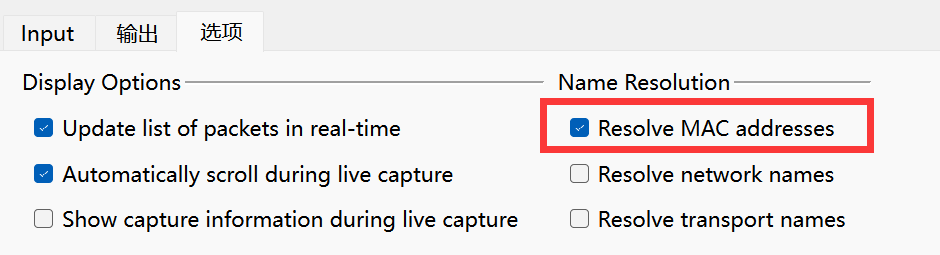
\includegraphics[width=0.4\textwidth]{lab2/rename.png}
  \caption{开启 Resolve MAC Addresses 选项}
  \label{fig:wireshark}
\end{figure}

\begin{figure} [H]
  \centering
  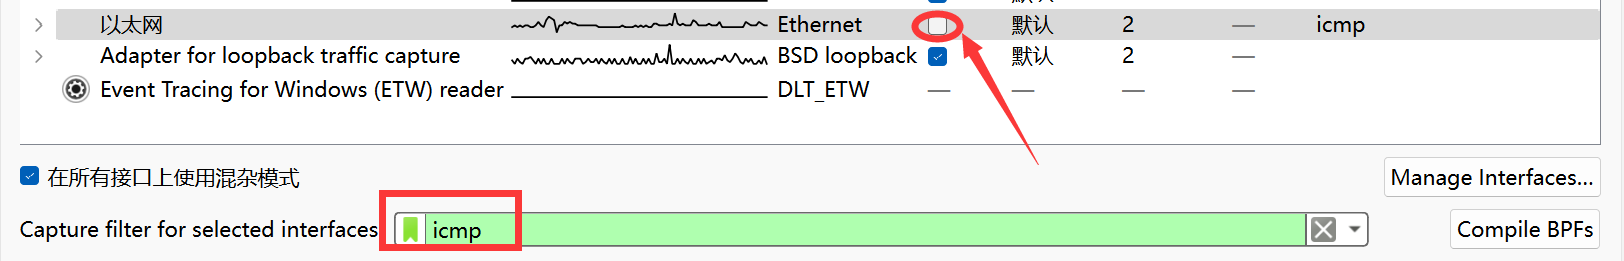
\includegraphics[width=0.6\textwidth]{lab2/icmp.png}
  \caption{开启 ICMP 捕获过滤器}
  \label{fig:icmp}
\end{figure}

\subsection{发送 ping 请求并捕获}

Wireshark 开始捕获后,用命令行向 www.baidu.com 发送 ping 请求。

\begin{figure} [H]
  \centering
  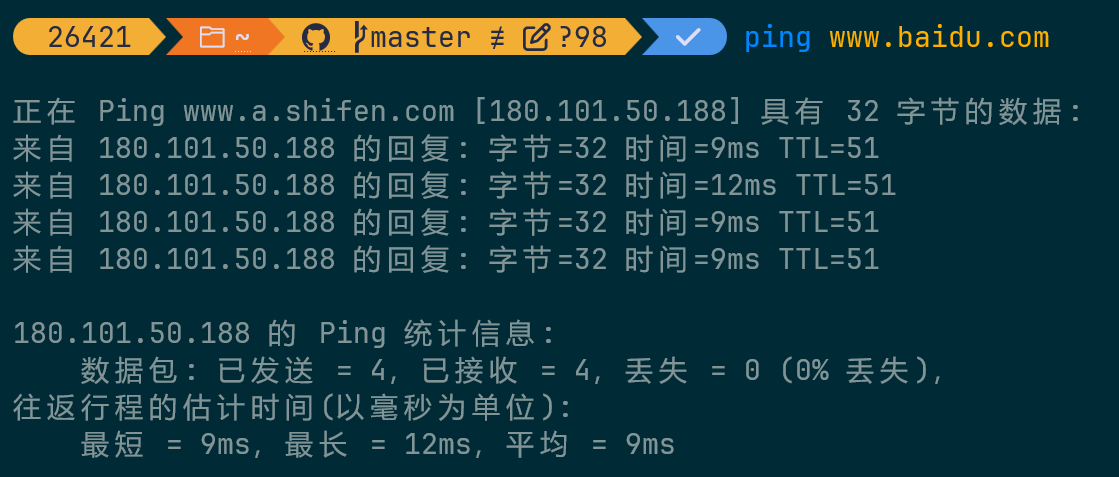
\includegraphics[width=0.45\textwidth]{lab2/ping.png}
  \label{fig:ping}
\end{figure}

由于这里的 ping 请求发送了四次数据包,所以在 Wireshark 中抓包也有四次响应 reply,
故我们随意选取一个 reply 进行分析即可。

\begin{figure}[H]
  \centering
  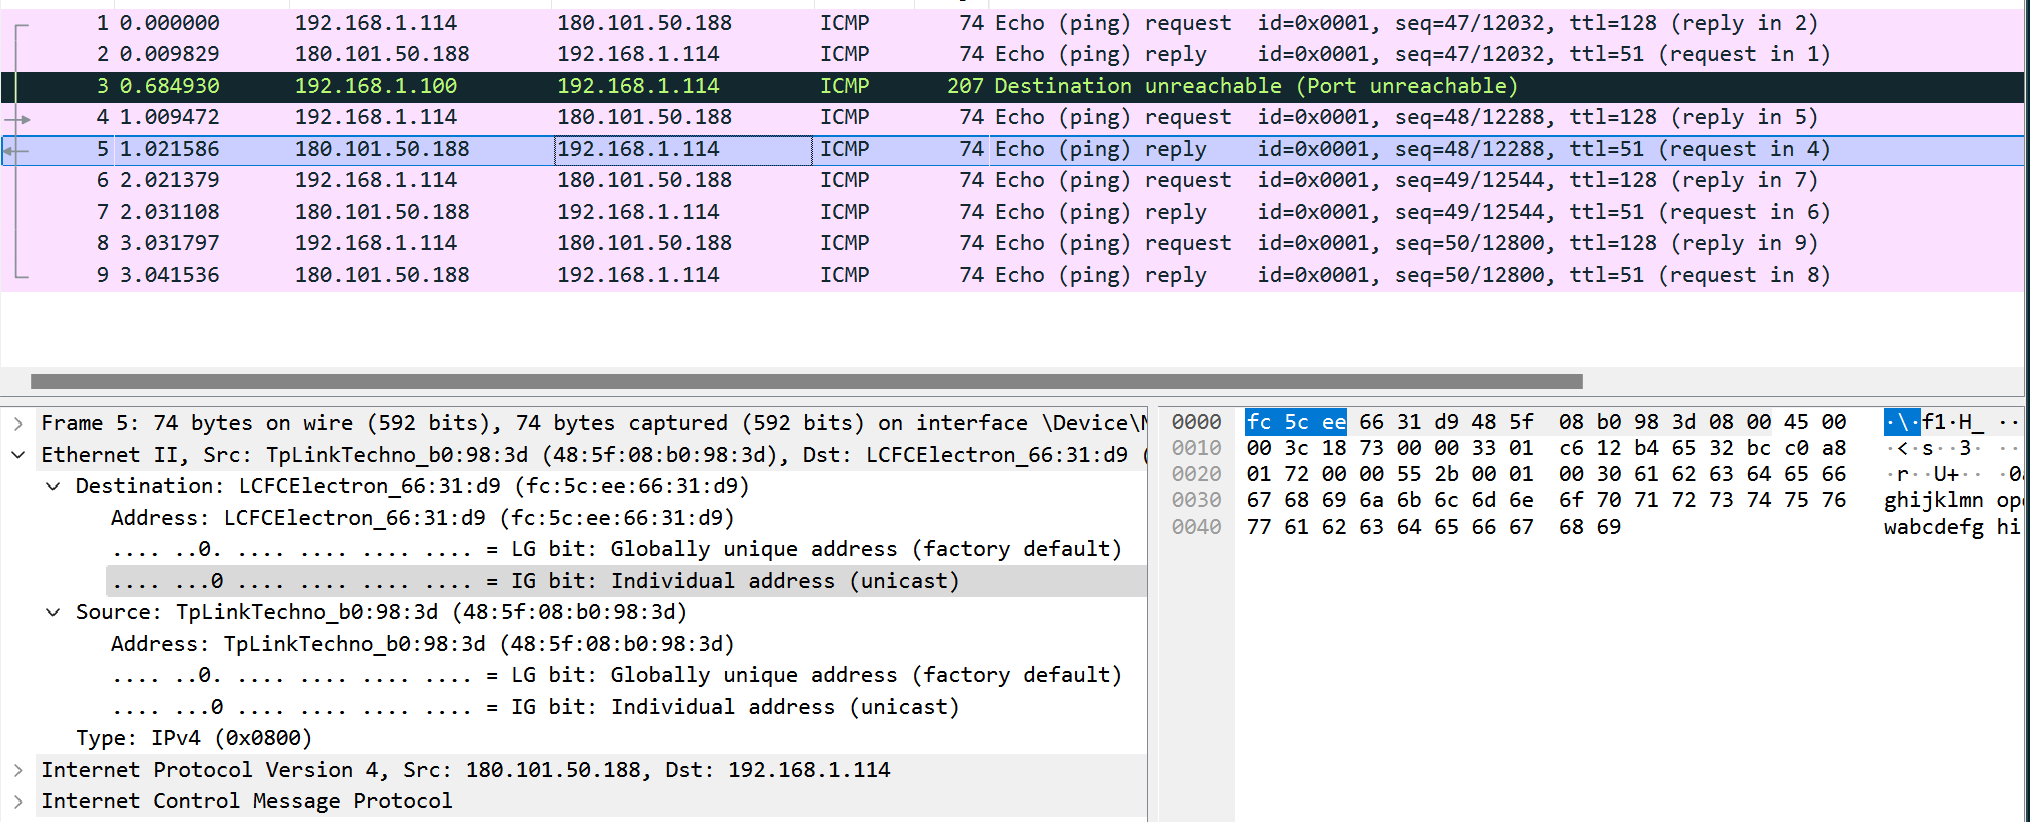
\includegraphics[width=0.68\textwidth]{lab2/wiresharkping.png}
  \caption{Wireshark 捕获的 ping 回复包}
  \label{fig:reply}
\end{figure}

在 Wireshark 中点击不同的字节,可以对应在左侧看到这部分的内容和意义。
要注意的是,大多数跟踪中都没有校验和,即使它确实存在。
通常,发送或接收帧的以太网硬件会计算或检查此字段,并添加或删除它。
因此,在大多数捕获设置中,操作系统或Wireshark根本看不到它。

\subsection{分析以太网帧结构}

我们左右对照,逐次点击不同的字段,便可以得出结果,下面是原图中各字段的含义:

\begin{figure} [H]
  \centering
  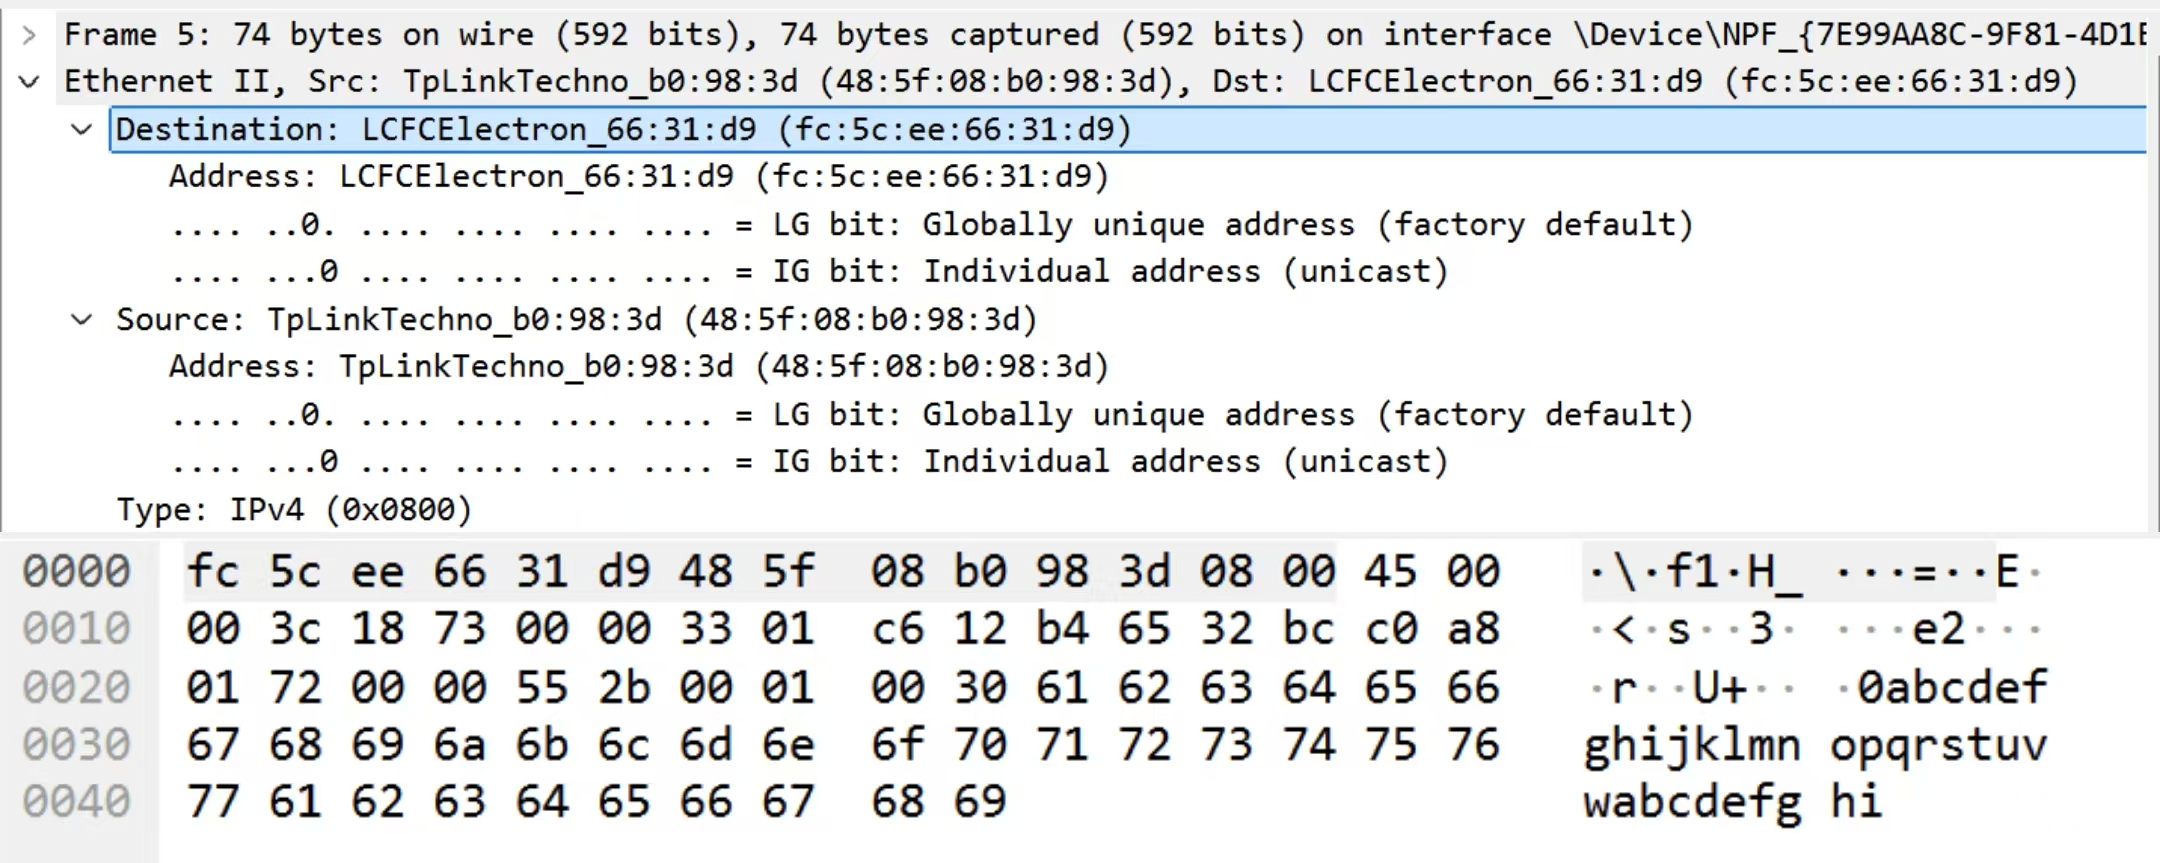
\includegraphics[width=0.6\textwidth]{lab2/combina.jpg}
  \caption{Combina}
  \label{fig:combina}
\end{figure}

现在,我们整理成以下的图片,以在一张图里显示帧结构:

\begin{figure} [H]
  \centering
  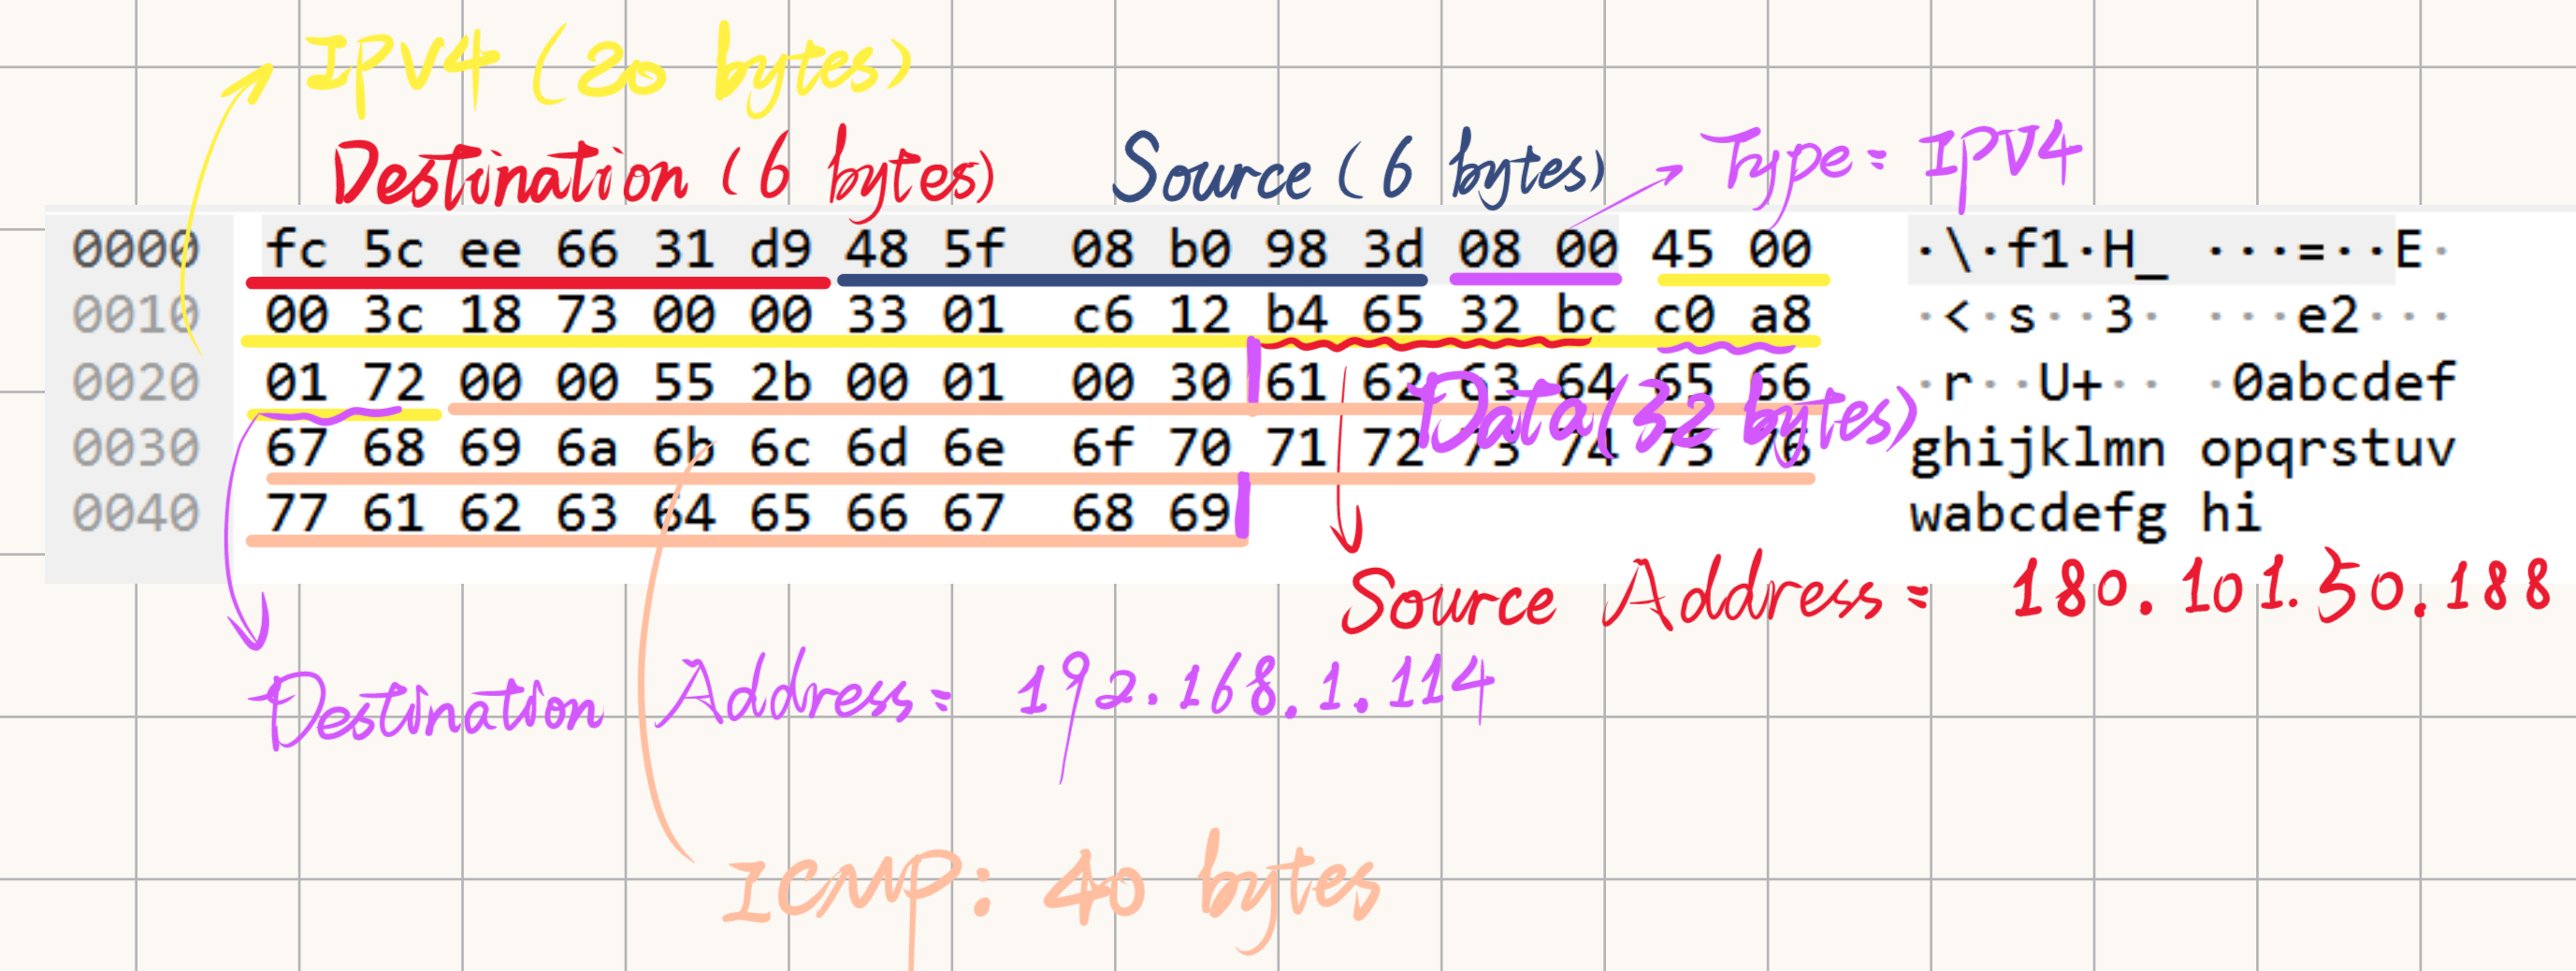
\includegraphics[width=0.75\textwidth]{lab2/structure.png}
  \caption{帧数据结构}
\end{figure}

在此图中,可见前 14 个字节为以太网的 Header,其中 Destination 和 Source 各占 6 字节,还剩下 2 字节为 Type 类型,这里是 IPV4.

接踵而至的是 IPV4 数据包,占有 20 个字节,其中体现了 Source Address 和 Destination Address,在此次抓包中,分别是 180.101.50.188 和 192.168.1.114。

后续跟随的是 ICMP 协议,共占 40 字节,其中用紫线分割开的是数据(32 Bytes)。

\begin{figure}[H]
  \centering
  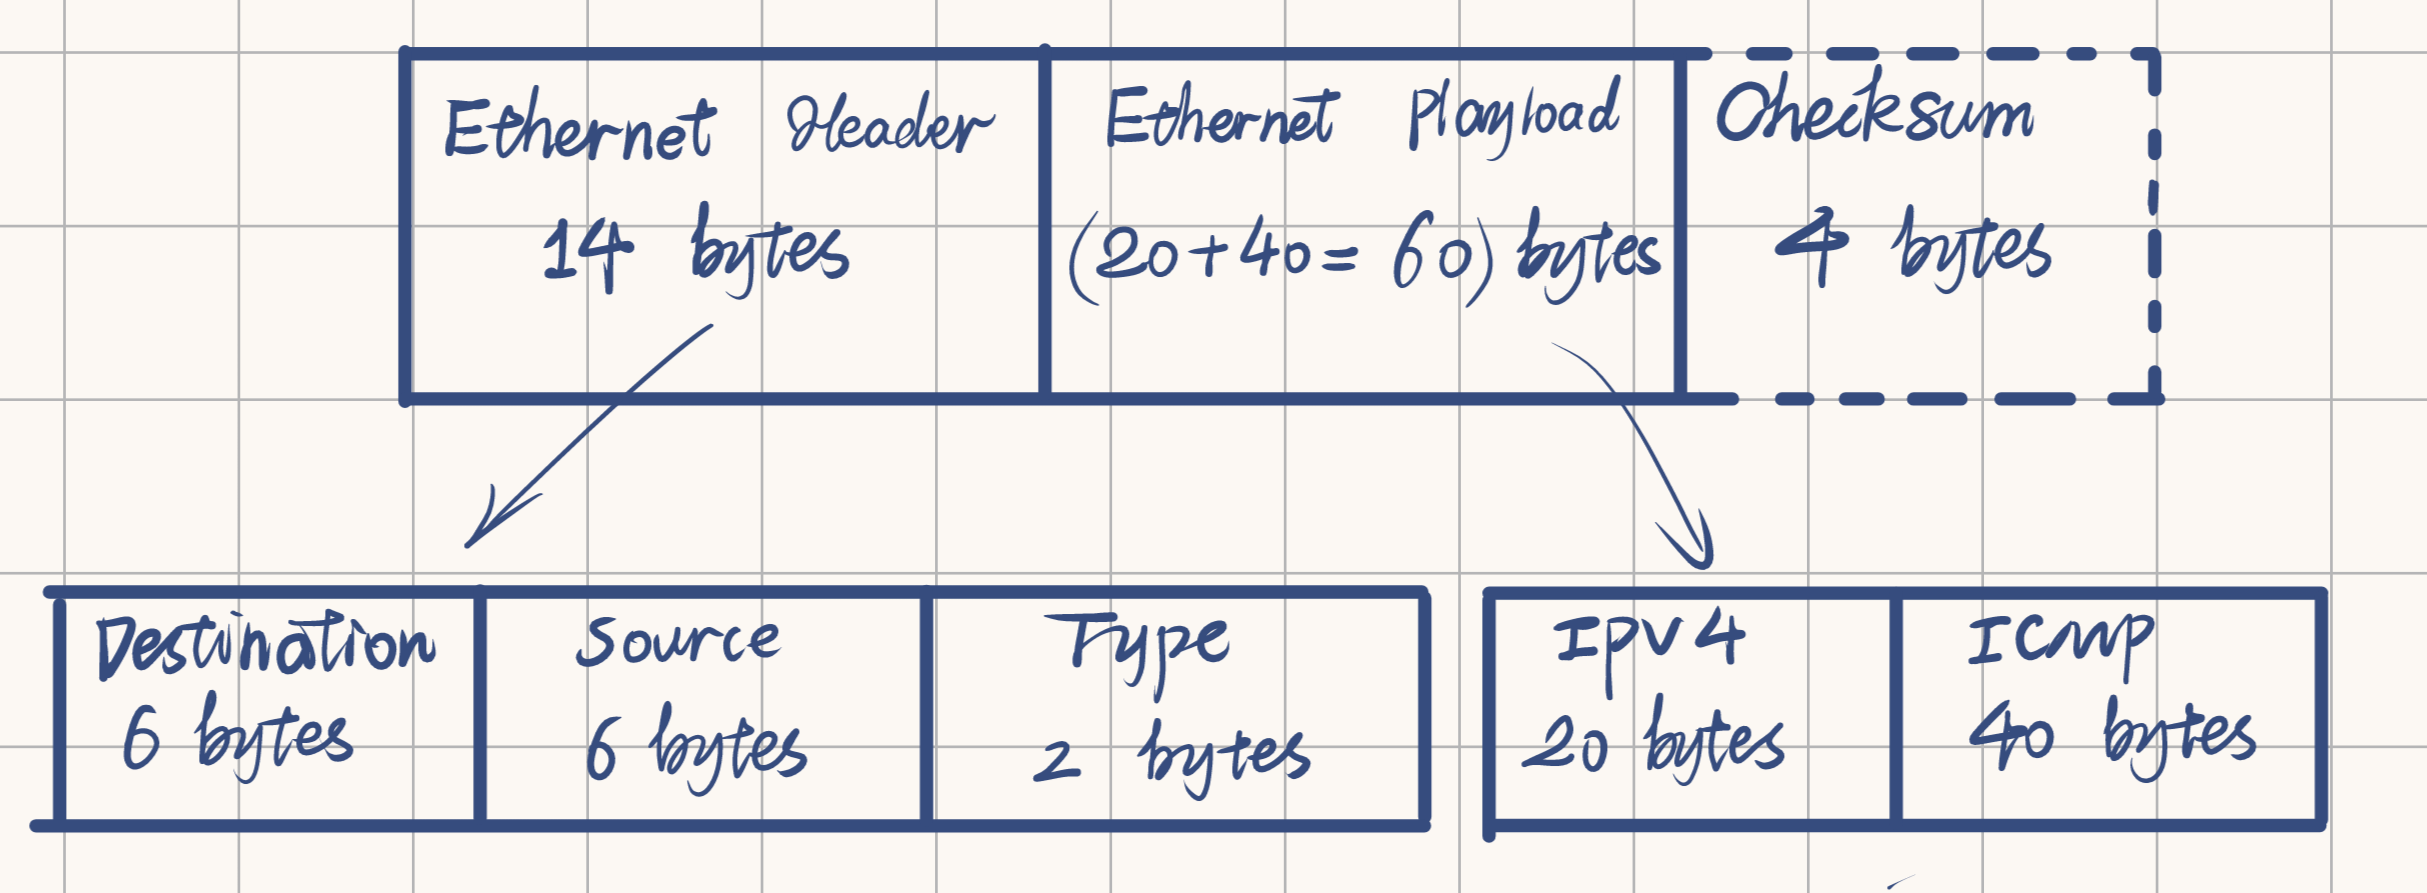
\includegraphics[width=0.6\textwidth]{lab2/draw.png}
  \caption{Structure}
\end{figure}

\subsection{Scope of Ethernet Addresses}

根据实验手册描述:

每个以太网帧都携带一个源地址和目标地址。其中一个地址是您的计算机地址。
它是发送帧的源,也是接收帧的目的地。
但另一个地址是什么?假设您ping了远程互联网服务器,
它不能是远程服务器的以太网地址,因为以太网帧只能寻址到一个局域网内。
相反,它将是路由器或默认网关的以太网地址,
例如802.11情况下的AP。这是将局域网连接到互联网其他部分的设备。
相比之下,每个数据包的IP块中的IP地址确实指示了整个源和目标端点。它们是您的计算机和远程服务器。

据此,以及上面分析获得的两个 IP 地址,可以画出以下的 Scope 图:

\begin{figure}[H]
  \centering
  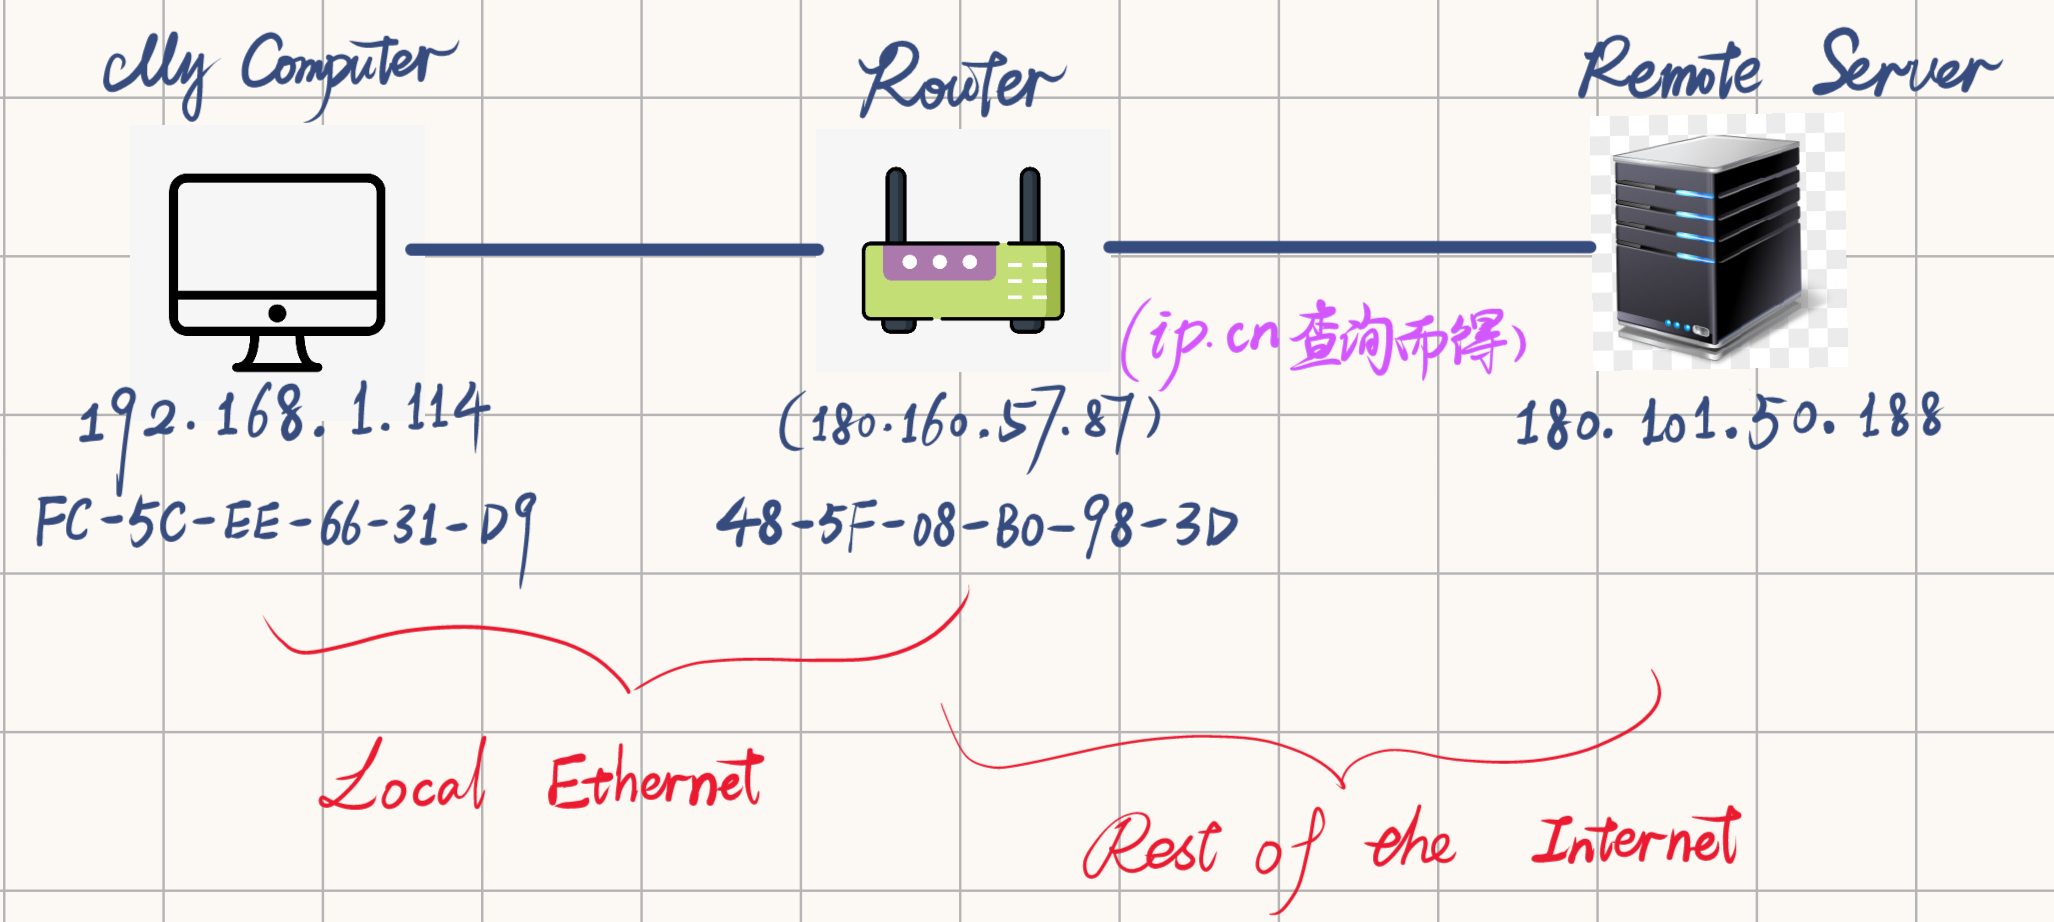
\includegraphics[width=0.5\textwidth]{lab2/scope.png}
  \caption{Scope}
\end{figure}

\subsection{Broadcast Frames}

为捕获以太网广播帧,需要重新抓包,在 Wireshark 中将 Filter 设置为 Ether Multicast,

\begin{figure}[H]
  \centering
  \includegraphics[width=0.6\textwidth]{lab2/Ether multicast.png}
  \caption{Ether Multicast}
\end{figure}

接下来,在命令行中使用 \texttt{ipconfig} 命令查询当前的 IP 地址:

\begin{figure}[H]
  \centering
  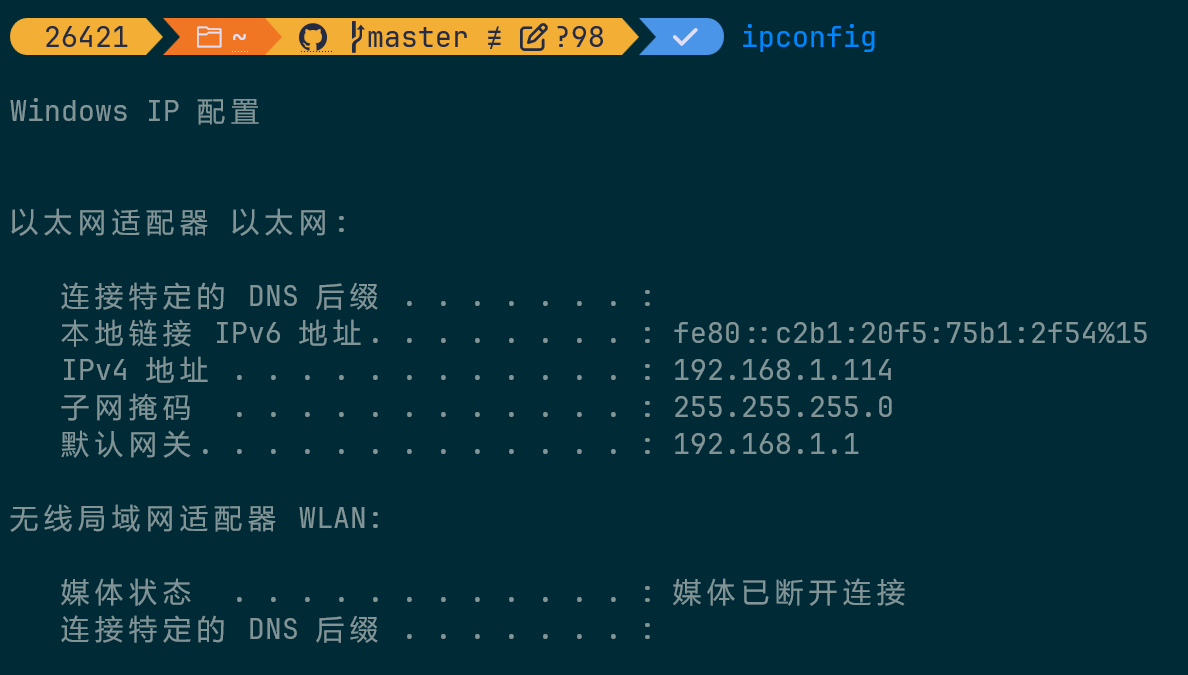
\includegraphics[width=0.4\textwidth]{lab2/ip.png}
  \caption{IP Config}
\end{figure}

然后 ping 本机地址,发送 Broadcast 广播帧:

\begin{figure}[H]
  \centering
  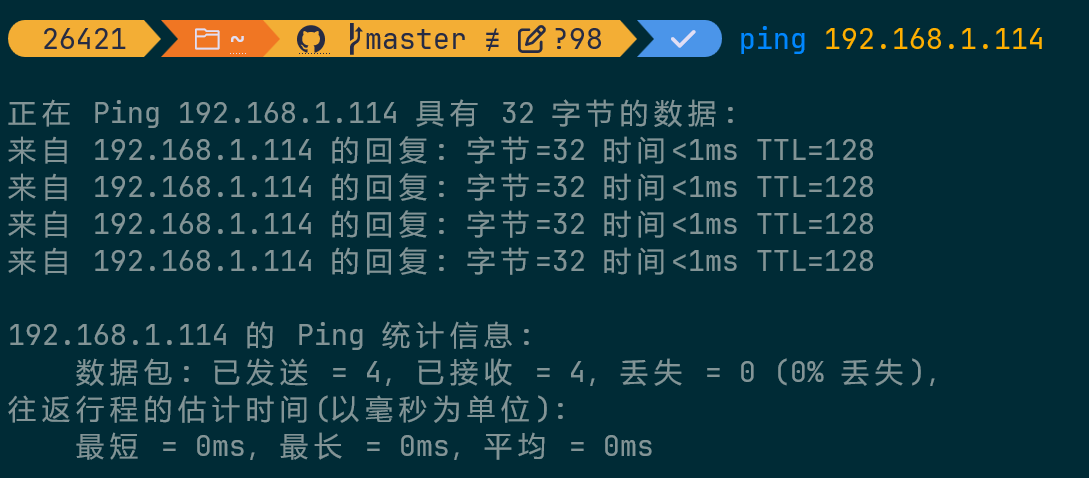
\includegraphics[width=0.4\textwidth]{lab2/broadcast.png}
  \caption{Broadcast}
\end{figure}

进入 Wireshark 查看捕获到的广播帧:

\begin{figure}[H]
  \centering
  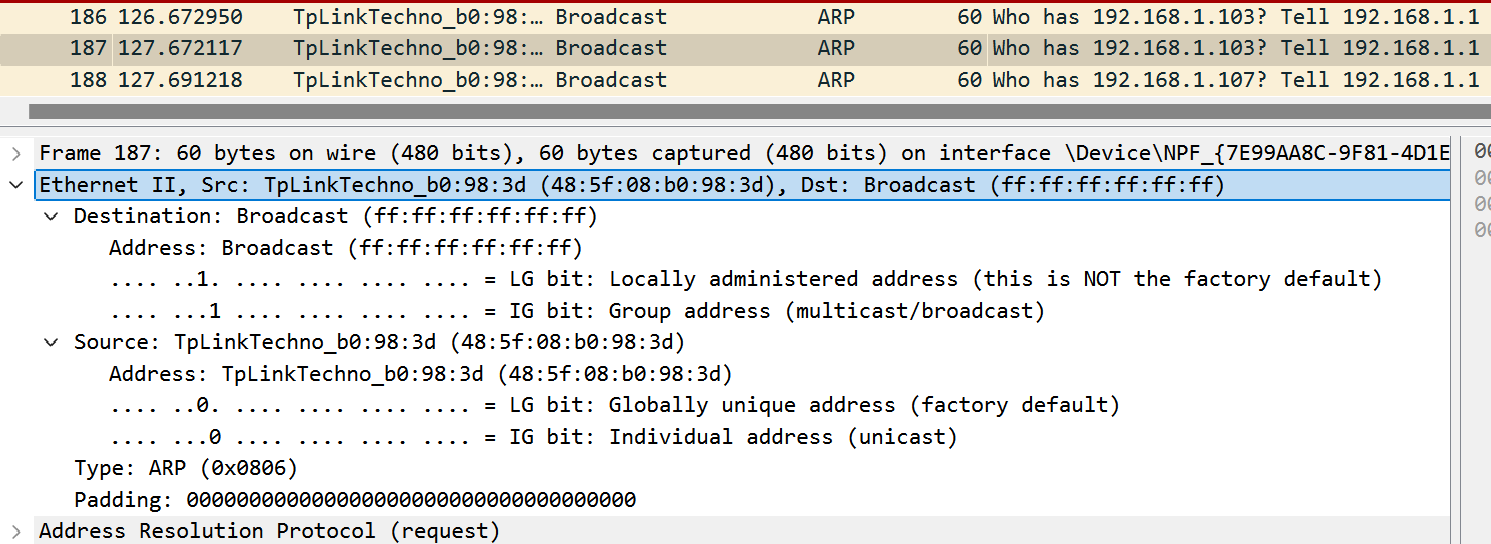
\includegraphics[width=0.65\textwidth]{lab2/wiresharkbroadcast.png}
  \caption{Wireshark Broadcast}
  \label{fig:wiresharkbroadcast}
\end{figure}

根据 Dst 的内容:\texttt{ff:ff:ff:ff:ff:ff},可以判断这是广播帧广播的地址。

根据下面这张图中提到的 IG bit: Group Address (multicast/broadcast)。

我们可以猜测,是这一位用来确定是单播或多播/广播。

至于为什么可以确定是这一位,可以看到 \ref{fig:wiresharkbroadcast} 图中,IG bit 在等于 0 和 1 时,后面括号表示了类型。

\begin{figure}[H]
  \centering
  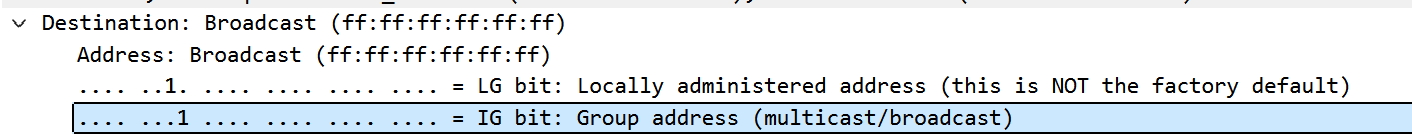
\includegraphics[width=0.6\textwidth]{lab2/brostcast.png}
  \caption{IG bit}
\end{figure}

所以,用 Wireshark 格式表达的以太网地址应该为:
\begin{lstlisting}
      .......1 ........ ........
\end{lstlisting}

\subsection{课后思考题}

通过解压 lab4stu.rar 获取 trace-ethernet.pcap 文件(在 Lab2 的实验指导手册中,示例图片就是打开了这个)。

用 Wireshark 打开,在上方的过滤器中搜索 llc,如下所示,弹出三个可选项。

\begin{figure}[H]
  \centering
  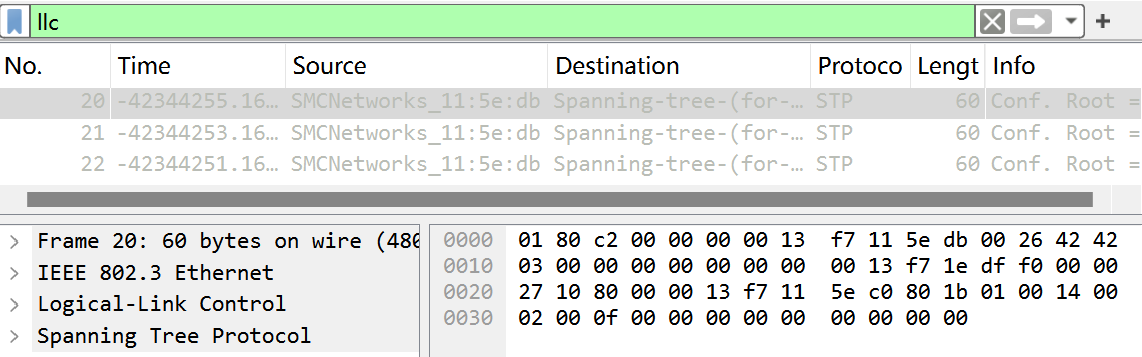
\includegraphics[width=0.6\textwidth]{lab2/llc.png}
  \caption{LLC}
\end{figure}



\subsubsection{Question 1}
How long are the combined IEEE 802.3 and LLC headers compared to the DIX Ethernet headers? You can use Wireshark to work this out. Note that the Trailer/Padding and Checksum may be shown as part of the header, but they come at the end of the frame.

与DIX以太网报头相比,IEEE 802.3和LLC组合报头有多长?您可以
使用Wireshark解决此问题。

请注意,Trailer / Padding 和 Checksum 可能显示为标头的一部分,但它们位于帧的末尾。

\subsubsection*{解答}
答: IEEE 802.3头为14个字节,与DIX以太网相同。

LLC又增加了3个字节的头,总共有17个字节的头。

\begin{figure}[H]
  \centering
  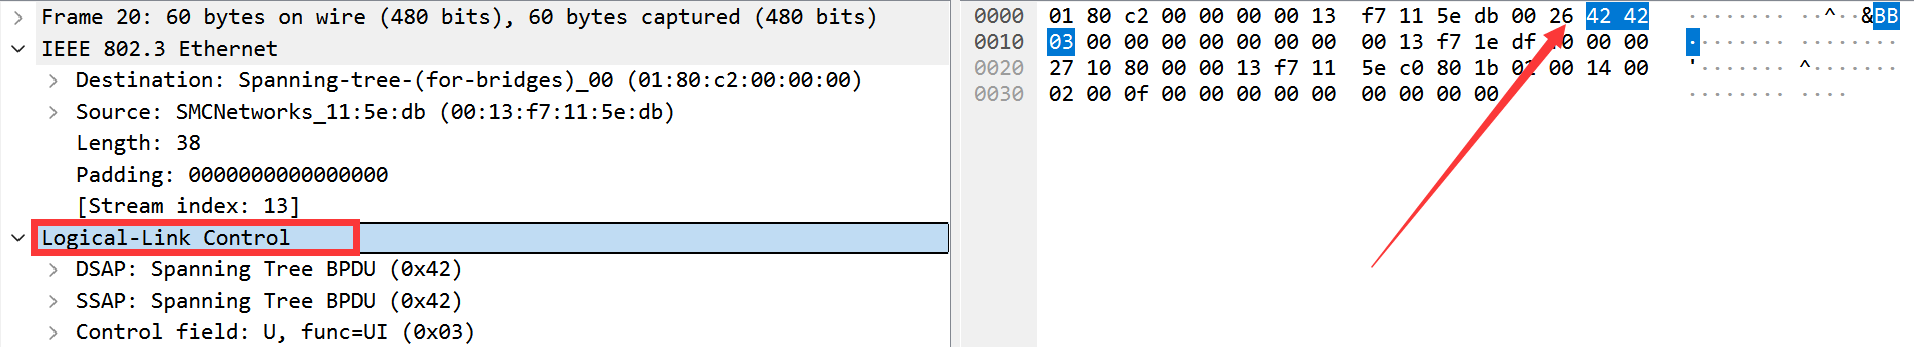
\includegraphics[width=0.6\textwidth]{lab2/llcmore.png}
  \caption{LLC}
\end{figure}

\subsubsection{Question 2}
How does the receiving computer know whether the frame is DIX Ethernet or IEEE 802.3? Hint: you may need to both use Wireshark to look at packet examples and read your text near where the Ethernet formats are described.

接收方计算机如何知道该帧是DIX以太网还是IEEE 802.3? 提示:
您可能需要同时使用Wireshark查看数据包示例并查找相关文献。

\subsubsection*{解答}
  参考资料:\href{https://www.globalknowledge.com/us-en/resources/resource-library/articles/what-is-the-difference-between-ethernet-ii-and-ieee-8023/}{WHAT IS THE DIFFERENCE BETWEEN ETHERNET II AND IEEE 802.3?}

如果帧头跟随 Source MAC 地址的 2 Bytes 的值大于 1536(0x600),则此 Frame 为 Ethernet II。
接着比较紧接着的 2 Bytes,如果为 0xFFFF 则为 Novell Ether 类型的 Frame ,
如果为 0xAAAA 则为 Ethernet SNAP 格式的 Frame , 如果都不是则为 Ethernet 802.3/802.2格式的帧。


\subsubsection{Question 3}
If IEEE 802.3 has no Type field, then how is the next higher layer determined? Use Wireshark to look for the demultiplexing key.

\subsubsection*{解答}

通过LLC中的信息确定下一层:读取DSAP和SSAP。

IEEE 802.3在IEEE 802.3报头之后紧接着添加LLC报头,以传达下一个更高的层协议。LLC使用
一个称为DSAP(目的服务接入点)的单一初始字节,而不是Type字段中的两个字节。

\begin{figure}[H]
  \centering
  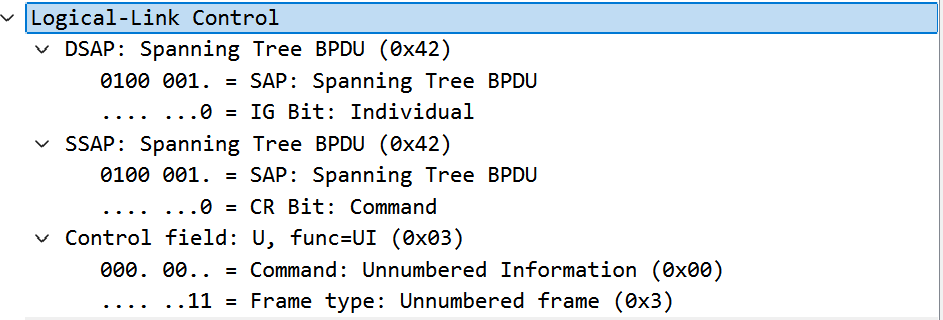
\includegraphics[width=0.6\textwidth]{lab2/DSAP.png}
  \caption{LLC Demux}
\end{figure}

\section{实验结果总结}

\subsection*{实验收获}

\begin{itemize}
  \item 本实验不仅加深了我对以太网帧结构的理解,还通过 Wireshark 工具提供了实践验证。
  \item 学会了如何通过抓包工具分析网络数据,为后续网络诊断及优化提供了实践基础。
  \item 通过分析广播帧、多播帧及单播帧的结构和用途,加深了对以太网地址分配和作用范围的理解。
\end{itemize}
  
\subsection*{实验不足和改进方向}

\begin{itemize}
  \item 在实验中,由于网络条件的限制,某些情况下捕获的数据量有限,未来可以尝试在更复杂的网络环境中进行类似实验。
  \item IEEE 802.3 的深入分析中,可以进一步尝试捕获更多类型的帧数据,以验证多种协议下的实际表现。
\end{itemize}

\section{附录}

\subsection*{参考资料}

\begin{itemize}
  \item \href{https://www.globalknowledge.com/us-en/resources/resource-library/articles/what-is-the-difference-between-ethernet-ii-and-ieee-8023/}{WHAT IS THE DIFFERENCE BETWEEN ETHERNET II AND IEEE 802.3?}
\end{itemize}

\end{document}